% ------------------- Aufgabe a -------------------
% R1: 67,23 \pm 0,1 (ohm)
% L: 16,87 \pm 0,05 (mH)
% positver Teil Parameter für Fit % y = a*exp(-b*x):
% a: 3,28805437898182
% b: 0,004658956201430903
% negativer Teil Parameter für Fit % y = -a*exp(-b*x):
% a: 3,195407081244171
% b: 0,0049642158489068555
% R_eff_exp: 0.0001623+/-0.0000005 (ohm)  (16,23 \pm 0,05) (mOhm)
% ------------------- Aufgabe b -------------------
% R_ap Theo: 5723+/-9 (ohm)
% ------------------- Aufgabe c -------------------
\section{Auswertung}
\label{sec:Auswertung}

\begin{figure}
  \centering
  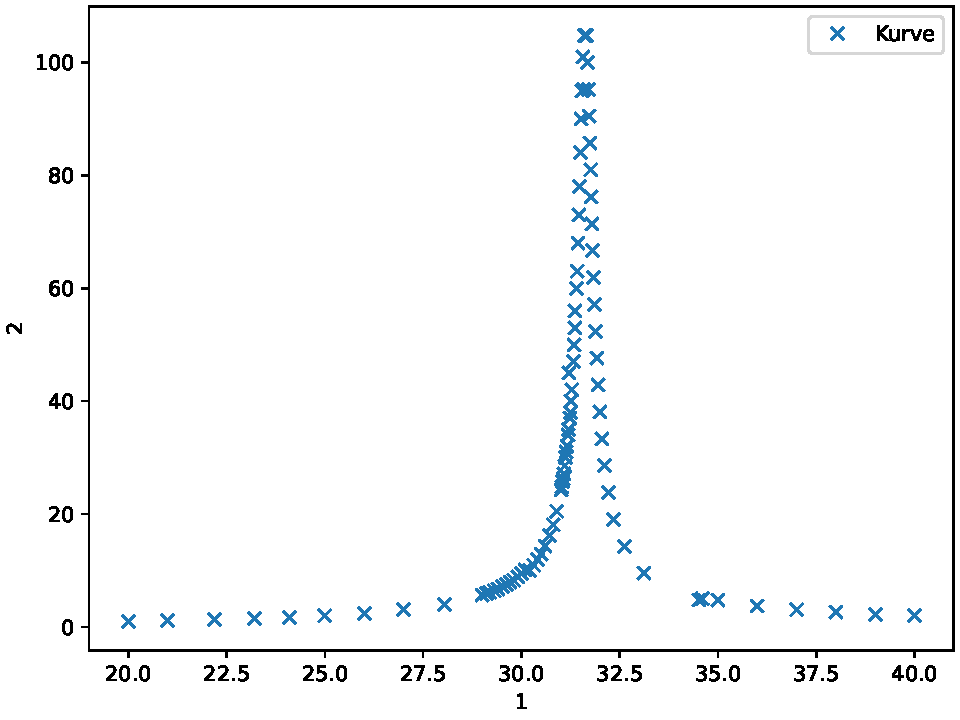
\includegraphics{plot.pdf}
  \caption{Plot.}
  \label{fig:plot}
\end{figure}

%Siehe \autoref{fig:plot}!